\documentclass[11pt,compress,t,notes=noshow, xcolor=table]{beamer}
\usepackage[]{graphicx}\usepackage[]{color}
% maxwidth is the original width if it is less than linewidth
% otherwise use linewidth (to make sure the graphics do not exceed the margin)
\makeatletter
\def\maxwidth{ %
  \ifdim\Gin@nat@width>\linewidth
    \linewidth
  \else
    \Gin@nat@width
  \fi
}
\makeatother

\newcommand{\citebutton}[2]{%
\beamergotobutton{\href{#2}{#1}}%
}

\newcommand{\blu}[1]{\textcolor{blue}{#1}}
\newcommand{\org}[1]{\textcolor{orange}{#1}}
\newcommand{\ques}{\textbf{\textcolor{red}{Question:  }}}
\newcommand{\questionssofar}{\begin{frame}\frametitle{Any questions?}\end{frame}}

\newcommand\warning{%
 \makebox[1.4em][c]{%
 \makebox[0pt][c]{\raisebox{.1em}{\scriptsize!}}%
 \makebox[0pt][c]{\color{red}\normalsize$\bigtriangleup$}}}%

\definecolor{fgcolor}{rgb}{0.345, 0.345, 0.345}
\newcommand{\hlnum}[1]{\textcolor[rgb]{0.686,0.059,0.569}{#1}}%
\newcommand{\hlstr}[1]{\textcolor[rgb]{0.192,0.494,0.8}{#1}}%
\newcommand{\hlcom}[1]{\textcolor[rgb]{0.678,0.584,0.686}{\textit{#1}}}%
\newcommand{\hlopt}[1]{\textcolor[rgb]{0,0,0}{#1}}%
\newcommand{\hlstd}[1]{\textcolor[rgb]{0.345,0.345,0.345}{#1}}%
\newcommand{\hlkwa}[1]{\textcolor[rgb]{0.161,0.373,0.58}{\textbf{#1}}}%
\newcommand{\hlkwb}[1]{\textcolor[rgb]{0.69,0.353,0.396}{#1}}%
\newcommand{\hlkwc}[1]{\textcolor[rgb]{0.333,0.667,0.333}{#1}}%
\newcommand{\hlkwd}[1]{\textcolor[rgb]{0.737,0.353,0.396}{\textbf{#1}}}%
\let\hlipl\hlkwb

\usepackage{framed}
\makeatletter
\newenvironment{kframe}{%
 \def\at@end@of@kframe{}%
 \ifinner\ifhmode%
  \def\at@end@of@kframe{\end{minipage}}%
  \begin{minipage}{\columnwidth}%
 \fi\fi%
 \def\FrameCommand##1{\hskip\@totalleftmargin \hskip-\fboxsep
 \colorbox{shadecolor}{##1}\hskip-\fboxsep
     % There is no \\@totalrightmargin, so:
     \hskip-\linewidth \hskip-\@totalleftmargin \hskip\columnwidth}%
 \MakeFramed {\advance\hsize-\width
   \@totalleftmargin\z@ \linewidth\hsize
   \@setminipage}}%
 {\par\unskip\endMakeFramed%
 \at@end@of@kframe}
\makeatother

\definecolor{shadecolor}{rgb}{.97, .97, .97}
\definecolor{messagecolor}{rgb}{0, 0, 0}
\definecolor{warningcolor}{rgb}{1, 0, 1}
\definecolor{errorcolor}{rgb}{1, 0, 0}
\newenvironment{knitrout}{}{} % an empty environment to be redefined in TeX

\usepackage{alltt}
\newcommand{\SweaveOpts}[1]{}  % do not interfere with LaTeX
\newcommand{\SweaveInput}[1]{} % because they are not real TeX commands
\newcommand{\Sexpr}[1]{}       % will only be parsed by R
\newcommand{\xmark}{\ding{55}}%


\usepackage[english]{babel}
\usepackage[utf8]{inputenc}

\usepackage{dsfont}
\usepackage{verbatim}
\usepackage{amsmath}
\usepackage{amsfonts}
\usepackage{amssymb}
\usepackage{bm}
\usepackage{csquotes}
\usepackage{multirow}
\usepackage{longtable}
\usepackage{booktabs}
\usepackage{enumerate}
\usepackage[absolute,overlay]{textpos}
\usepackage{psfrag}
\usepackage{algorithm}
\usepackage{algpseudocode}
\usepackage{eqnarray}
\usepackage{arydshln}
\usepackage{tabularx}
\usepackage{placeins}
\usepackage{tikz}
\usepackage{setspace}
\usepackage{colortbl}
\usepackage{mathtools}
\usepackage{wrapfig}
\usepackage{bm}
\usepackage{amsmath}
\usepackage{pifont}

\usetikzlibrary{shapes.multipart,shapes,arrows,automata,positioning,calc,chains,trees, shadows}
\tikzset{
  %Define standard arrow tip
  >=stealth',
  %Define style for boxes
  punkt/.style={
    rectangle,
    rounded corners,
    draw=black, very thick,
    text width=6.5em,
    minimum height=2em,
    text centered},
  % Define arrow style
  pil/.style={
    ->,
    thick,
    shorten <=2pt,
    shorten >=2pt,}
}

\tikzstyle{vec}=[draw, rectangle, fill = white, minimum width=5mm, minimum height=1cm, inner sep = 2pt]

\usepackage{subfig}

% Defines macros and environments
\usepackage{../../style/lmu-lecture}


\let\code=\texttt
\let\proglang=\textsf

\setkeys{Gin}{width=0.9\textwidth}

\setbeamertemplate{frametitle}{\expandafter\uppercase\expandafter\insertframetitle}

\usepackage{bbm}
% basic latex stuff
\newcommand{\pkg}[1]{{\fontseries{b}\selectfont #1}} %fontstyle for R packages
\newcommand{\lz}{\vspace{0.5cm}} %vertical space
\newcommand{\dlz}{\vspace{1cm}} %double vertical space
\newcommand{\oneliner}[1] % Oneliner for important statements
{\begin{block}{}\begin{center}\begin{Large}#1\end{Large}\end{center}\end{block}}


%new environments
\newenvironment{vbframe}  %frame with breaks and verbatim
{
 \begin{frame}[containsverbatim,allowframebreaks]
}
{
\end{frame}
}

\newenvironment{vframe}  %frame with verbatim without breaks (to avoid numbering one slided frames)
{
 \begin{frame}[containsverbatim]
}
{
\end{frame}
}

\newenvironment{blocki}[1]   % itemize block
{
 \begin{block}{#1}\begin{itemize}
}
{
\end{itemize}\end{block}
}

\newenvironment{fragileframe}[2]{  %fragile frame with framebreaks
\begin{frame}[allowframebreaks, fragile, environment = fragileframe]
\frametitle{#1}
#2}
{\end{frame}}


\newcommand{\myframe}[2]{  %short for frame with framebreaks
\begin{frame}[allowframebreaks]
\frametitle{#1}
#2
\end{frame}}

\newcommand{\remark}[1]{
  \textbf{Remark:} #1
}


\newenvironment{deleteframe}
{
\begingroup
\usebackgroundtemplate{
\includegraphics[width=\paperwidth,height=\paperheight]{../style/color/red.png}}
 \begin{frame}
}
{
\end{frame}
\endgroup
}
\newenvironment{simplifyframe}
{
\begingroup
\usebackgroundtemplate{
\includegraphics[width=\paperwidth,height=\paperheight]{../style/color/yellow.png}}
 \begin{frame}
}
{
\end{frame}
\endgroup
}\newenvironment{draftframe}
{
\begingroup
\usebackgroundtemplate{
\includegraphics[width=\paperwidth,height=\paperheight]{../style/color/green.jpg}}
 \begin{frame}
}
{
\end{frame}
\endgroup
}
% https://tex.stackexchange.com/a/261480: textcolor that works in mathmode
\makeatletter
\renewcommand*{\@textcolor}[3]{%
  \protect\leavevmode
  \begingroup
    \color#1{#2}#3%
  \endgroup
}
\makeatother





\input{../../latex-math/basic-math.tex}
\input{../../latex-math/basic-ml.tex}


\newcommand{\titlefigure}{figure/err_surf}
\newcommand{\learninggoals}{
\item Understand how the risk function is optimized to
  learn the optimal parameters of a model
\item Understand the idea of gradient descent as a basic risk optimizer}

\title{Introduction to Machine Learning}
\date{}

\begin{document}

\lecturechapter{ML-Basics: Optimization}
\lecture{Introduction to Machine Learning}


\begin{vbframe}{Learning as Parameter Optimization}
\begin{itemize}
\item We have seen, we can operationalize the search for a model $f$ that matches
    training data best, by looking for its parametrization $\thetab \in \Theta$
    with lowest empirical risk $\risket$.
\item Therefore, we usually traverse the error surface downwards; often by local search from a starting point to its minimum.
\end{itemize}
\begin{center}
\begin{figure}[!b]
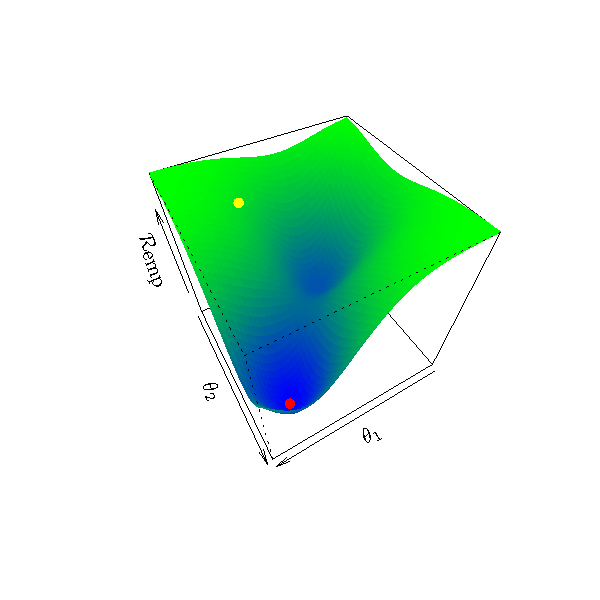
\includegraphics[trim=2.4cm 2.4cm 2.4cm 2.4cm, width=0.4\textwidth]{figure/err_surf}
\end{figure}
\end{center}

\framebreak

The ERM optimization problem is:
% this means that we find the best model $\hat f$ parametrized by parameters $\thetabh \in \Theta$ regarding an empirical risk $\riske$ by \textbf{minimizing} $\risket$ with respect to $\thetab$, i.e., 

\[
\thetabh  = \argmin_{\thetab \in \Theta} \risket .
\]

For a \textbf{(global) minimum} $\thetabh$ it obviously holds that 
\[
\forall \thetab \in \Theta :\quad \riske(\thetabh) \leq \risket .
\]

This does not imply that $\thetabh$ is unique. \\
\lz
Which kind of numerical technique is reasonable for this problem strongly depends 
on model and parameter structure (continuous params? uni-modal $\risket$?). 
Here, we will only discuss very simple scenarios.

\end{vbframe}
\begin{vbframe}{Local Minima}

If $\riske$ is continuous in $\thetab$ we can define a \textbf{local minimum} $\thetabh$:
\[
\exists \epsilon > 0\; \forall \thetab \text{ with } \left\Vert\thetabh - \thetab\right\Vert < \epsilon: \quad \riske(\thetabh) \leq \risket .
\]
Clearly every global minimum is also a local minimum.
Finding a local minimum is easier than finding a global minimum.

\begin{center}
\begin{figure}[!b]
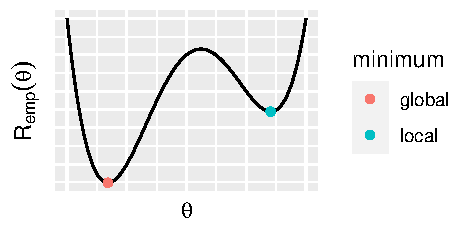
\includegraphics[width=0.7\textwidth]{figure/g_l_min}
\end{figure}
\end{center}

\end{vbframe}
\begin{vbframe}{Local Minima and stationary points}
\footnotesize
If $\riske$ is continuously differentiable in $\thetab$ then a \textbf{sufficient condition} for a local minimum is that $\thetabh$ is \textbf{stationary} with 0 gradient, so no local improvement is possible:
\[
\frac{\partial}{\partial\thetab}\riske(\thetabh) = 0
\]
and the Hessian $\frac{\partial^2}{\partial\thetab^2}\riske(\thetabh)$ is positive definite. While the neg. gradient points into the direction of fastest local decrease, the Hessian measures local curvature of $\riske$.

\begin{figure}[!htb]
\minipage{0.32\textwidth}
  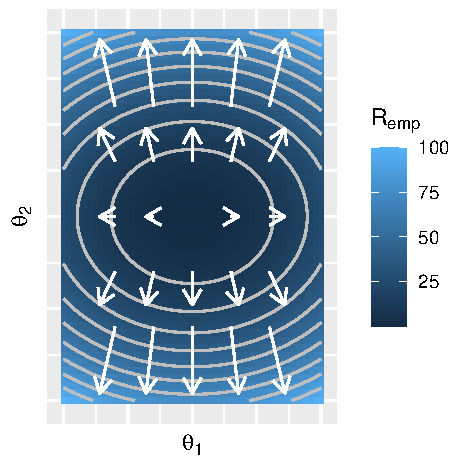
\includegraphics[width=\linewidth]{figure/grad}
  \caption*{\footnotesize$\frac{\partial}{\partial\thetab}\riske(\thetab)$}
\endminipage\hfill
\minipage{0.32\textwidth}
  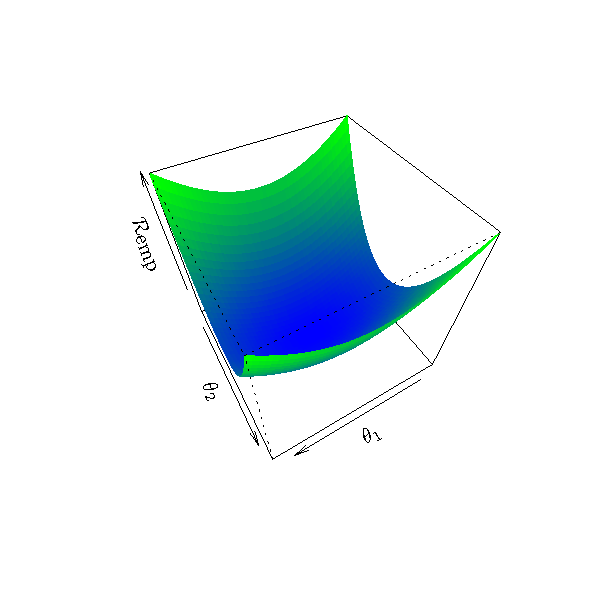
\includegraphics[trim=2.2cm 2.2cm 2.2cm 2.2cm, width=\linewidth]{figure/hess1}
  \caption*{\footnotesize const. pos. def. Hessian}
\endminipage\hfill
\minipage{0.32\textwidth}%
  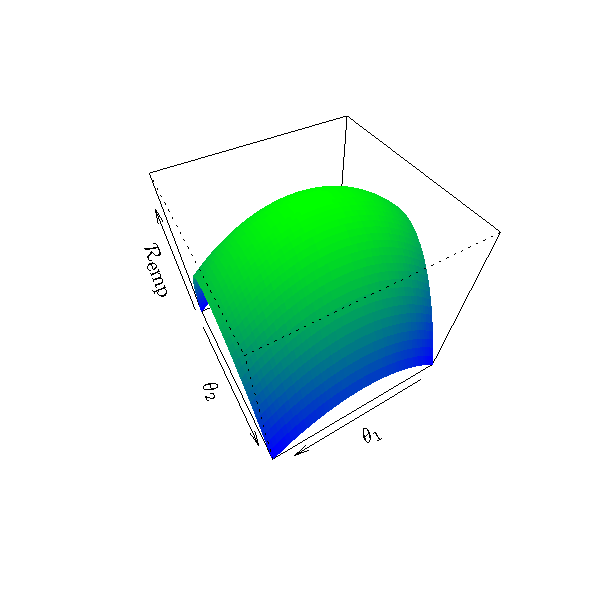
\includegraphics[trim=2.2cm 2.2cm 2.2cm 2.2cm, width=\linewidth]{figure/hess2}
  \caption*{\footnotesize const. neg. def. Hessian}
\endminipage
\end{figure}

\end{vbframe}
\begin{vbframe}{Least Squares Estimator}
Now, for given features $\Xmat \in \mathbb{R}^{n\times p}$ and target $\yv \in \mathbb{R}^n$, we want to find the best linear model regarding the squared error loss, i.e.,
\[\risket = \left\Vert \Xmat\thetab - \yv\right\Vert_2^2 = \sumin (\thetab^\top\xv^{(i)} - \yi)^2\;.\]

With the sufficient condition for continously differentiable functions it can be shown that the \textbf{least squares estimator}
\[\thetabh = (\Xmat^\top\Xmat)^{-1}\Xmat^\top\yv.\]
is a local minimum of $\riske$. If $\Xmat$ is full-rank, $\riske$ is strictly convex and there is only one local minimum - which is also global. \\

\lz \textbf{Note:} Often such analytical solutions in ML are not possible, and we rather have to use iterative numerical optimization.

\end{vbframe}
\begin{vbframe}{Gradient Descent}
    The simple idea of GD is to iteratively go from the current candidate $\thetab^{[t]}$ in the direction of the negative gradient, i.e., the direction of the steepest descent, with learning rate $\alpha$ to the next $\thetab^{[t+1]}$:
\[
    \thetab^{[t+1]} = \thetab^{[t]} - \alpha \frac{\partial}{\partial\thetab}{\riske(\thetab^{[t]})}.
\]

\begin{tabular}{l}

\minipage{0.32\textwidth}
  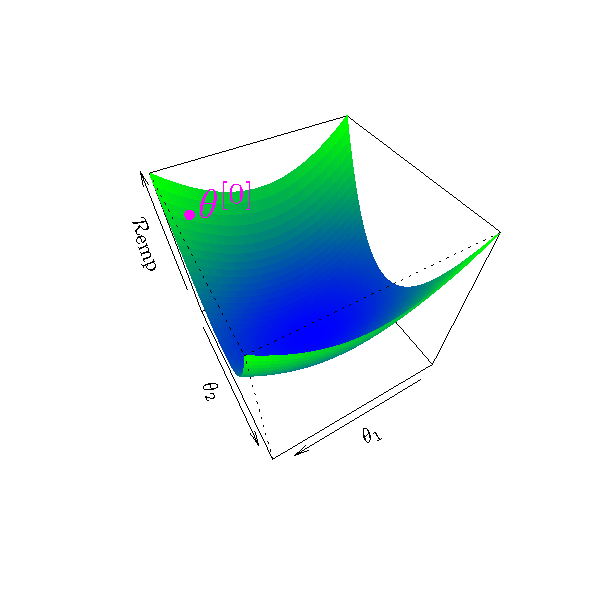
\includegraphics[trim=2cm 2cm 2cm 2cm, width=\linewidth]{figure/grad_desc1}  
\endminipage\hfill
\minipage{0.1\textwidth}
$\;$
\endminipage\hfill
\minipage{0.54\textwidth}
\vspace{0pt}% 
We choose a random start $\thetab^{[0]}$ with risk $\riske(\thetab^{[0]}) = 76.25.$
\endminipage\hfill
\end{tabular}

\end{vbframe}

\begin{vbframe}{Gradient Descent - Example}
\begin{tabular}{l}
\minipage{0.32\textwidth}
  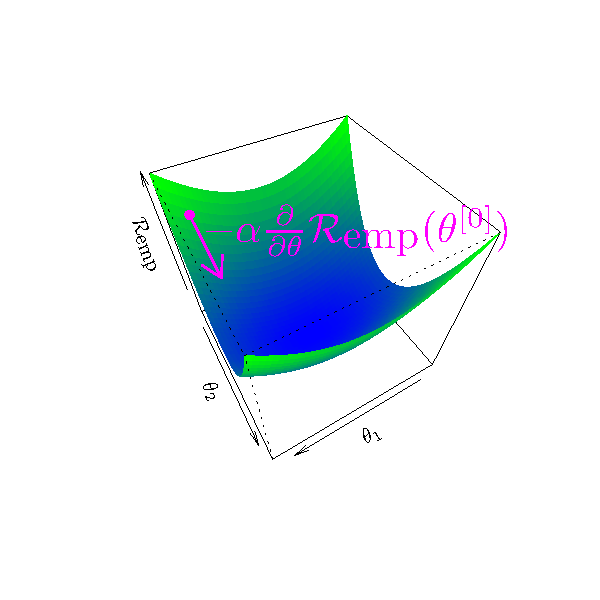
\includegraphics[trim=2cm 2cm 2cm 2cm, width=\linewidth]{figure/grad_desc2}  
\endminipage\hfill
\minipage{0.1\textwidth}
$\;$
\endminipage\hfill
\minipage{0.54\textwidth}
\vspace{0pt}% 
Now we follow in the direction of the negative gradient at $\thetab^{[0]}$.
\endminipage\hfill
\\
\minipage{0.32\textwidth}
  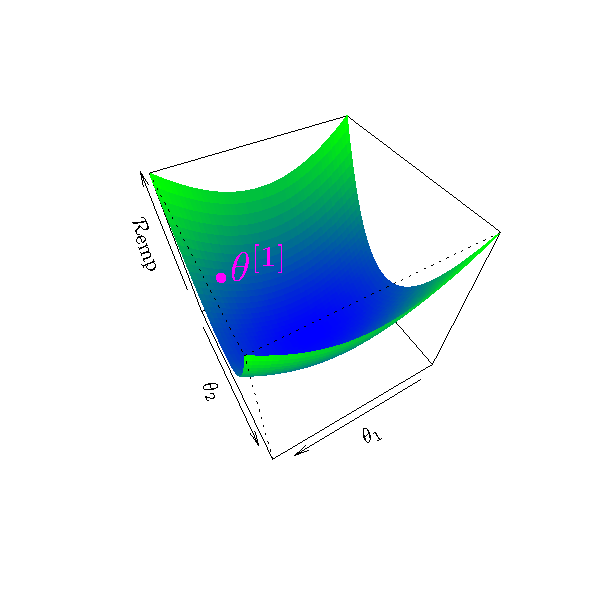
\includegraphics[trim=2cm 2cm 2cm 2cm, width=\linewidth]{figure/grad_desc3}  
\endminipage\hfill
\minipage{0.1\textwidth}
$\;$
\endminipage\hfill
\minipage{0.54\textwidth}
\vspace{0pt}% 
We arrive at $\thetab^{[1]}$ with risk\\$\riske(\thetab^{[1]}) \approx 42.73.$ \\ We improved:\\$\riske(\thetab^{[1]}) < \riske(\thetab^{[0]}).$
\endminipage\hfill
\end{tabular}
\end{vbframe}
\begin{vbframe}{Gradient Descent - Example}
\begin{tabular}{l}
\minipage{0.32\textwidth}
  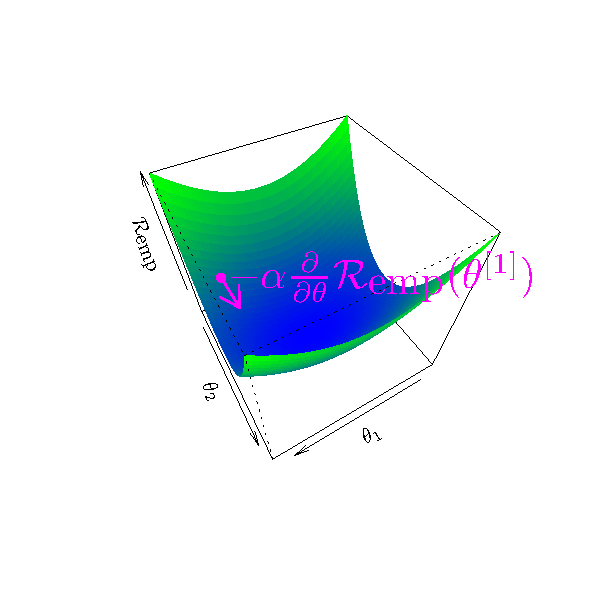
\includegraphics[trim=2cm 2cm 2cm 2cm, width=\linewidth]{figure/grad_desc4}  
\endminipage\hfill
\minipage{0.1\textwidth}
$\;$
\endminipage\hfill
\minipage{0.54\textwidth}
\vspace{0pt}% 
Again we follow in the direction of the negative gradient, but now at $\thetab^{[1]}.$
\endminipage\hfill
\\
\minipage{0.32\textwidth}
  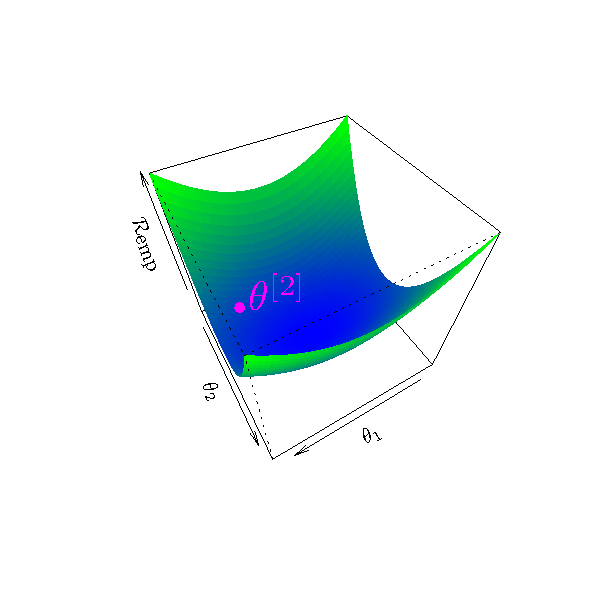
\includegraphics[trim=2cm 2cm 2cm 2cm, width=\linewidth]{figure/grad_desc5}  
\endminipage\hfill
\minipage{0.1\textwidth}
$\;$
\endminipage\hfill
\minipage{0.54\textwidth}
\vspace{0pt}% 
Now $\thetab^{[2]}$ has risk $\riske(\thetab^{[2]}) \approx 25.08.$
% Thus clearly, we have improved our estimation again.
\endminipage\hfill
\end{tabular}
\end{vbframe}
\begin{vbframe}{Gradient Descent - Example}
\begin{tabular}{l}
\minipage{0.32\textwidth}
  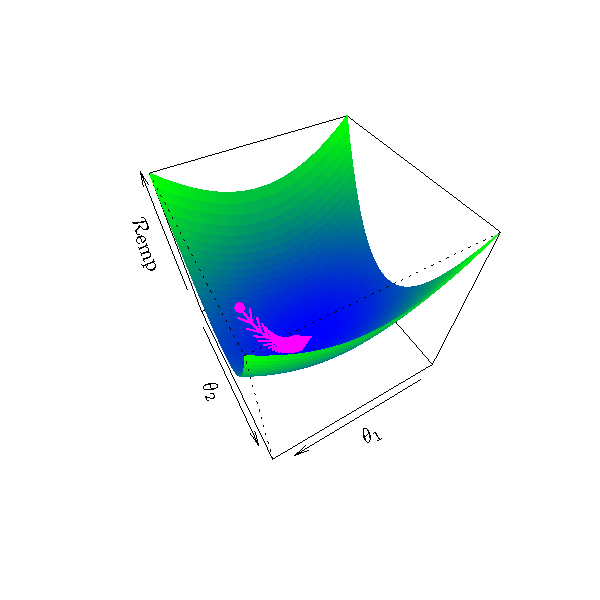
\includegraphics[trim=2cm 2cm 2cm 2cm, width=\linewidth]{figure/grad_desc6}  
\endminipage\hfill
\minipage{0.1\textwidth}
$\;$
\endminipage\hfill
\minipage{0.54\textwidth}
\vspace{0pt}% 
We iterate this until some form of convergence or termination.
% \footnote[frame]{This is not the only stopping criterium; e.g., we could limit the number of iterations.}. 
\endminipage\hfill
\\
\minipage{0.32\textwidth}
  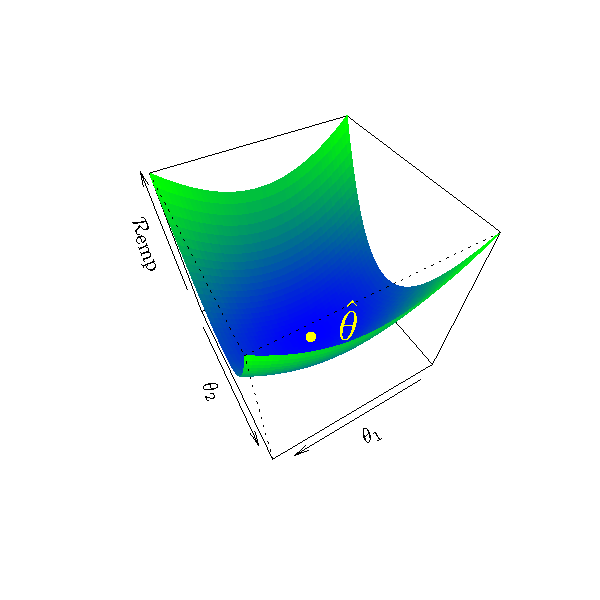
\includegraphics[trim=2cm 2cm 2cm 2cm, width=\linewidth]{figure/grad_desc7}  
\endminipage\hfill
\minipage{0.1\textwidth}
$\;$
\endminipage\hfill
\minipage{0.54\textwidth}
\vspace{0pt}% 
We arrive close to a stationary $\thetabh$ which is hopefully at least
a local minimum.
\endminipage\hfill
\end{tabular}
\end{vbframe}

\begin{vbframe}{Gradient Descent - Learning Rate}
\footnotesize
\begin{itemize}
\item The negative gradient is a direction that looks locally promising to reduce $\riske$. \\
\item Hence it weights components higher
    % \footnote[frame]{in an absolute sense} 
    in which $\riske$ decreases more. \\
\item However, the length of $-\frac{\partial}{\partial\thetab}{\riske}$ measures only the local decrease rate, i.e., there are no guarantees that we will not go "too far". \\
\item We use a learning rate $\alpha$ to scale the step length in each iteration. Too much can lead to overstepping and no converge, too low leads to slow convergence.
\item Usually, a simple constant rate or rate-decrease mechanisms to enforce local convergence are used
    % control the rate. 
\end{itemize}
\begin{figure}[!htb]
\minipage{0.32\textwidth}
  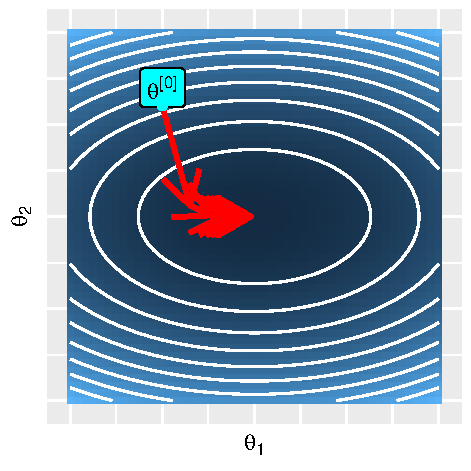
\includegraphics[width=\linewidth]{figure/grad_desc_alpha1}
  \caption*{\tiny good convergence for $\alpha_1$}
\endminipage\hfill
\minipage{0.32\textwidth}
  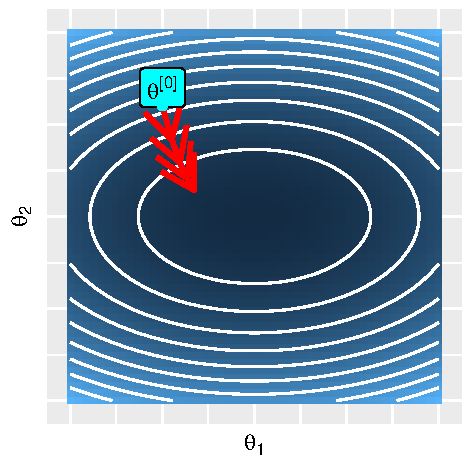
\includegraphics[width=\linewidth]{figure/grad_desc_alpha2}
  \caption*{\tiny poor convergence for $\alpha_2 (< \alpha_1$)}
\endminipage\hfill
\minipage{0.32\textwidth}%
  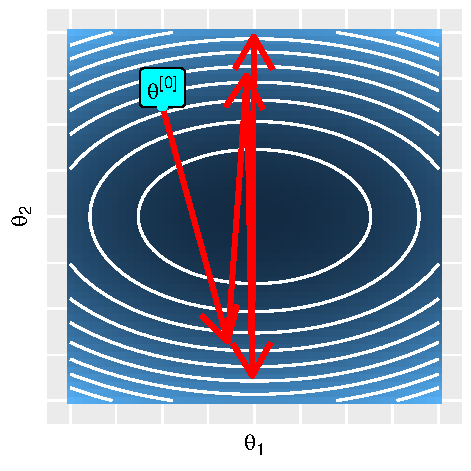
\includegraphics[width=\linewidth]{figure/grad_desc_alpha3}
  \caption*{\tiny no convergence for $\alpha_3 (> \alpha_1$)}
\endminipage
\end{figure}

\end{vbframe}

\begin{vbframe}{Further topics}
\begin{itemize}
\item GD is a so-called first-order method. Second-order methods use the Hessian to refine the search direction for faster convergence.
\item There exist many improvements of GD, e.g., to smartly control the learn rate, to escape saddle points, to mimic second order behavior without computing the expensive Hessian.
    % ould also optimize the learning rate $\alpha$.
% \item If some parameters are dependent of each other, we can model such dependicies either by \textbf{equality} or \textbf{inequality constraints}, i.e., 
% \[g(\thetab) = 0 \quad \text{or} \quad h(\thetab) \geq 0.\]
% There exist numerical methods to solve constrained optimization problems, such as sequential quadratic programming.
\item If the gradient of GD is not derived from the empirical risk of the whole data set, but instead from a randomly selected subset, we call this \textbf{stochastic gradient descent} (SGD). For large-scale problems this can lead to higher computational efficiency.
% \item Often it is desirable to not allow arbitrarily large $\Vert \thetabh \Vert$, since this could result, among other things, in numerical instability of the method. This procedure is called \textbf{regularization}.
\end{itemize}
\end{vbframe}


% \begin{vbframe}{Further topics}
    % learning vs optimuzation,.,.,.
% \end{vbframe}


\endlecture

\end{document}
